\begin{figure}[H]
\raggedleft
	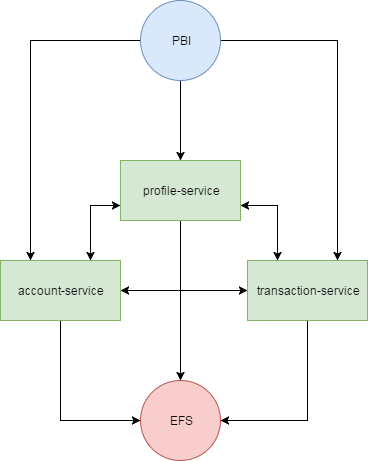
\includegraphics[scale=0.5]{images/travailNeuflizeOBC/architecture/pbiEfs.png}
	\centering
	\caption{Composition des services EFS}
	\label{coucheMicroservices}
\end{figure}

L'API microservices utilise la stack Netflix OSS qui permet d'intégrer les patterns classiques aux application distribuées. Les composants Netflix sont intégrés via Spring Cloud. Les principales briques techniques de l'API sont les suivantes :\\

\begin{itemize}
	\item Un serveur de configuration basé sur Archaius
	\item Un serveur d'annuaire basé sur Eureka
	\item Une gateway implémentée via Zuul
	\item Trois services métiers :
		\begin{itemize}
			\item account-service : gérant les informations liées aux comptes des utilisateurs
			\item profile-service : gérant les informations liées aux profils des utilisateurs
			\item transaction-service : gérant les informations liées aux transactions bancaires
		\end{itemize}
	\item Une interface d'analyses des logs pour le monitoring basée sur la stack ELK : ElasticSearch, Logstash et kibana
	\item Un dashboard basé sur Zipkin
\end{itemize}